\section{Results}
To begin, an overall overview of the results was conducted. In Figure \ref{fig:Scorespaper}, the paper-level score comparison revealed substantial variability across individual studies, with the differences between human and LLMs evaluations varying considerably from one paper to another, rather than following a consistent pattern.
\vspace{-0.5cm}
\begin{figure}[H]
    \centering
    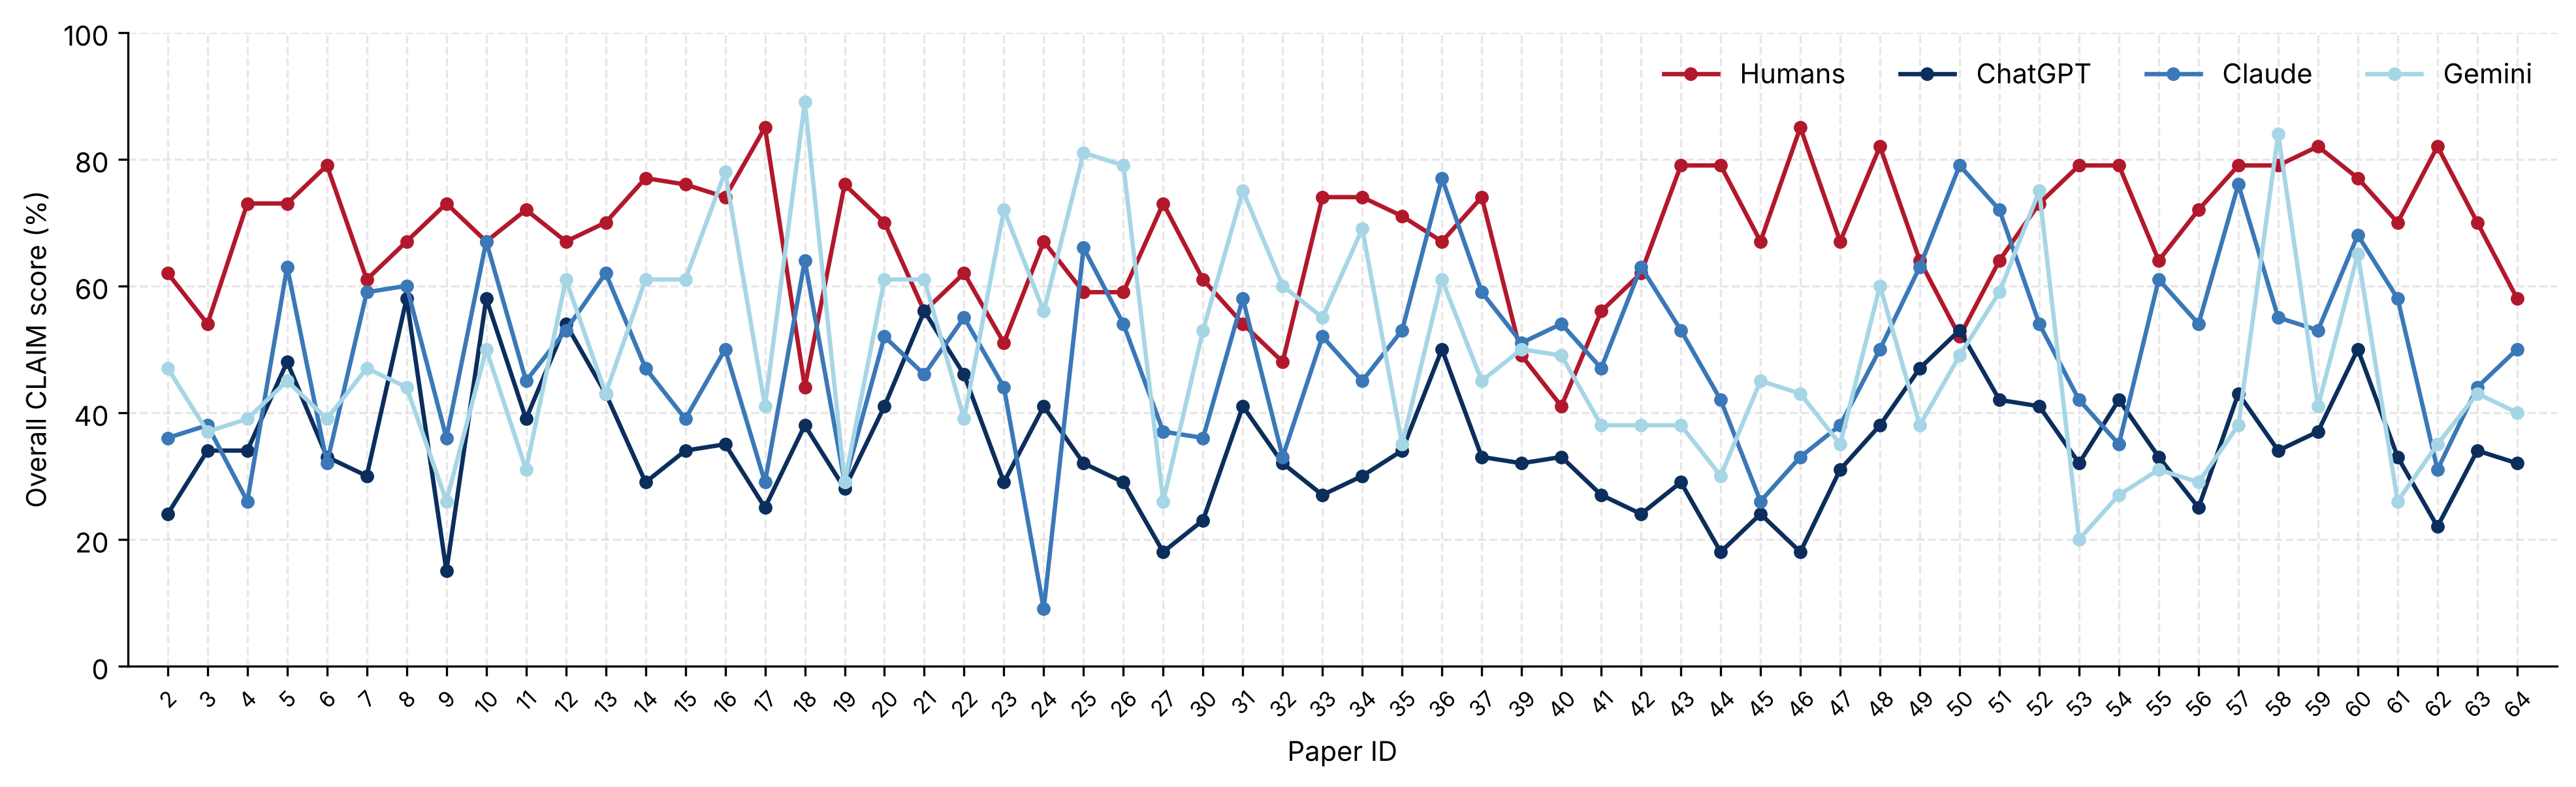
\includegraphics[width=0.8\linewidth]{images/35ScoresResults2.png}
    \caption{Comparison of CLAIM overall scores assigned by humans and LLMs.}
    \label{fig:Scorespaper}
\end{figure}
\vspace{-0.5cm}
\noindent
The boxplots in Figure \ref{fig:scoreDistribution} showed  the majority of human evaluations were between 62-77\%. The three LLMs gave lower and more dispersed scores for the majority of the observations: ChatGPT had a range of 28–41\%, Gemini of 38–61\% and Claude of 38–59\%. 

As it can be seen in bar plots in Figure \ref{fig:scoreDomain}, human evaluators gave the highest mean compliance to Model description (87.00\%) and the lowest to Dataset description (61.70\%). LLMs had their lowest-scored domain in Model description, for ChatGPT (19.17\%) and Claude (29.63\%); Gemini was the exception (57.42\%). In contrast, Performance became the highest-scored domain for all three LLMs (67.98-77.47\%), exceeding the human score (64.00\%). 
\vspace{-0.5cm}
\begin{figure}[H]
    \centering
    \captionsetup[subfigure]{font=scriptsize}
    \begin{subfigure}{0.38\linewidth}
        \centering
        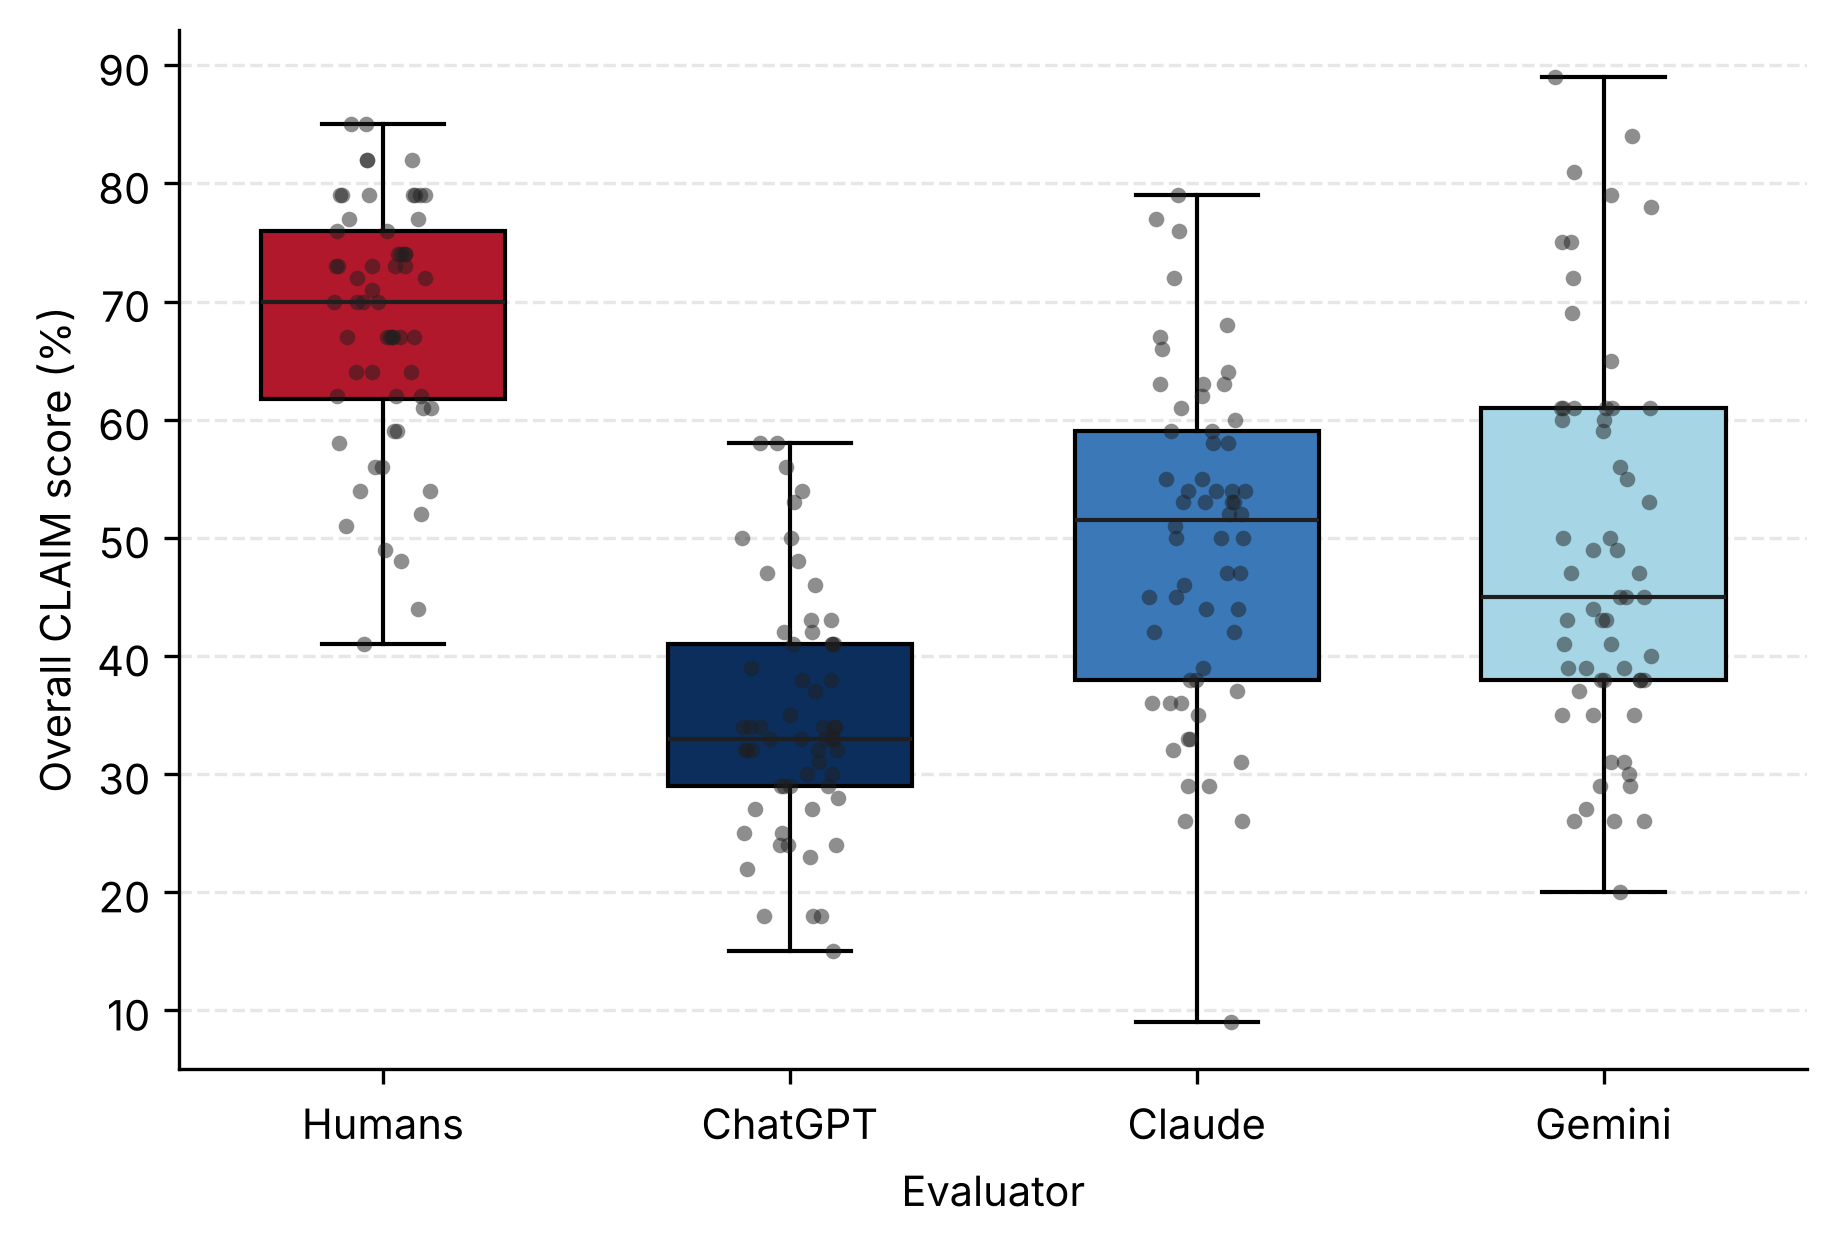
\includegraphics[height=3cm]{images/4ScoresDistribution2.png}
        \caption{}
        \label{fig:scoreDistribution}
    \end{subfigure}
    \hfill
    \begin{subfigure}{0.52\linewidth}
        \centering
        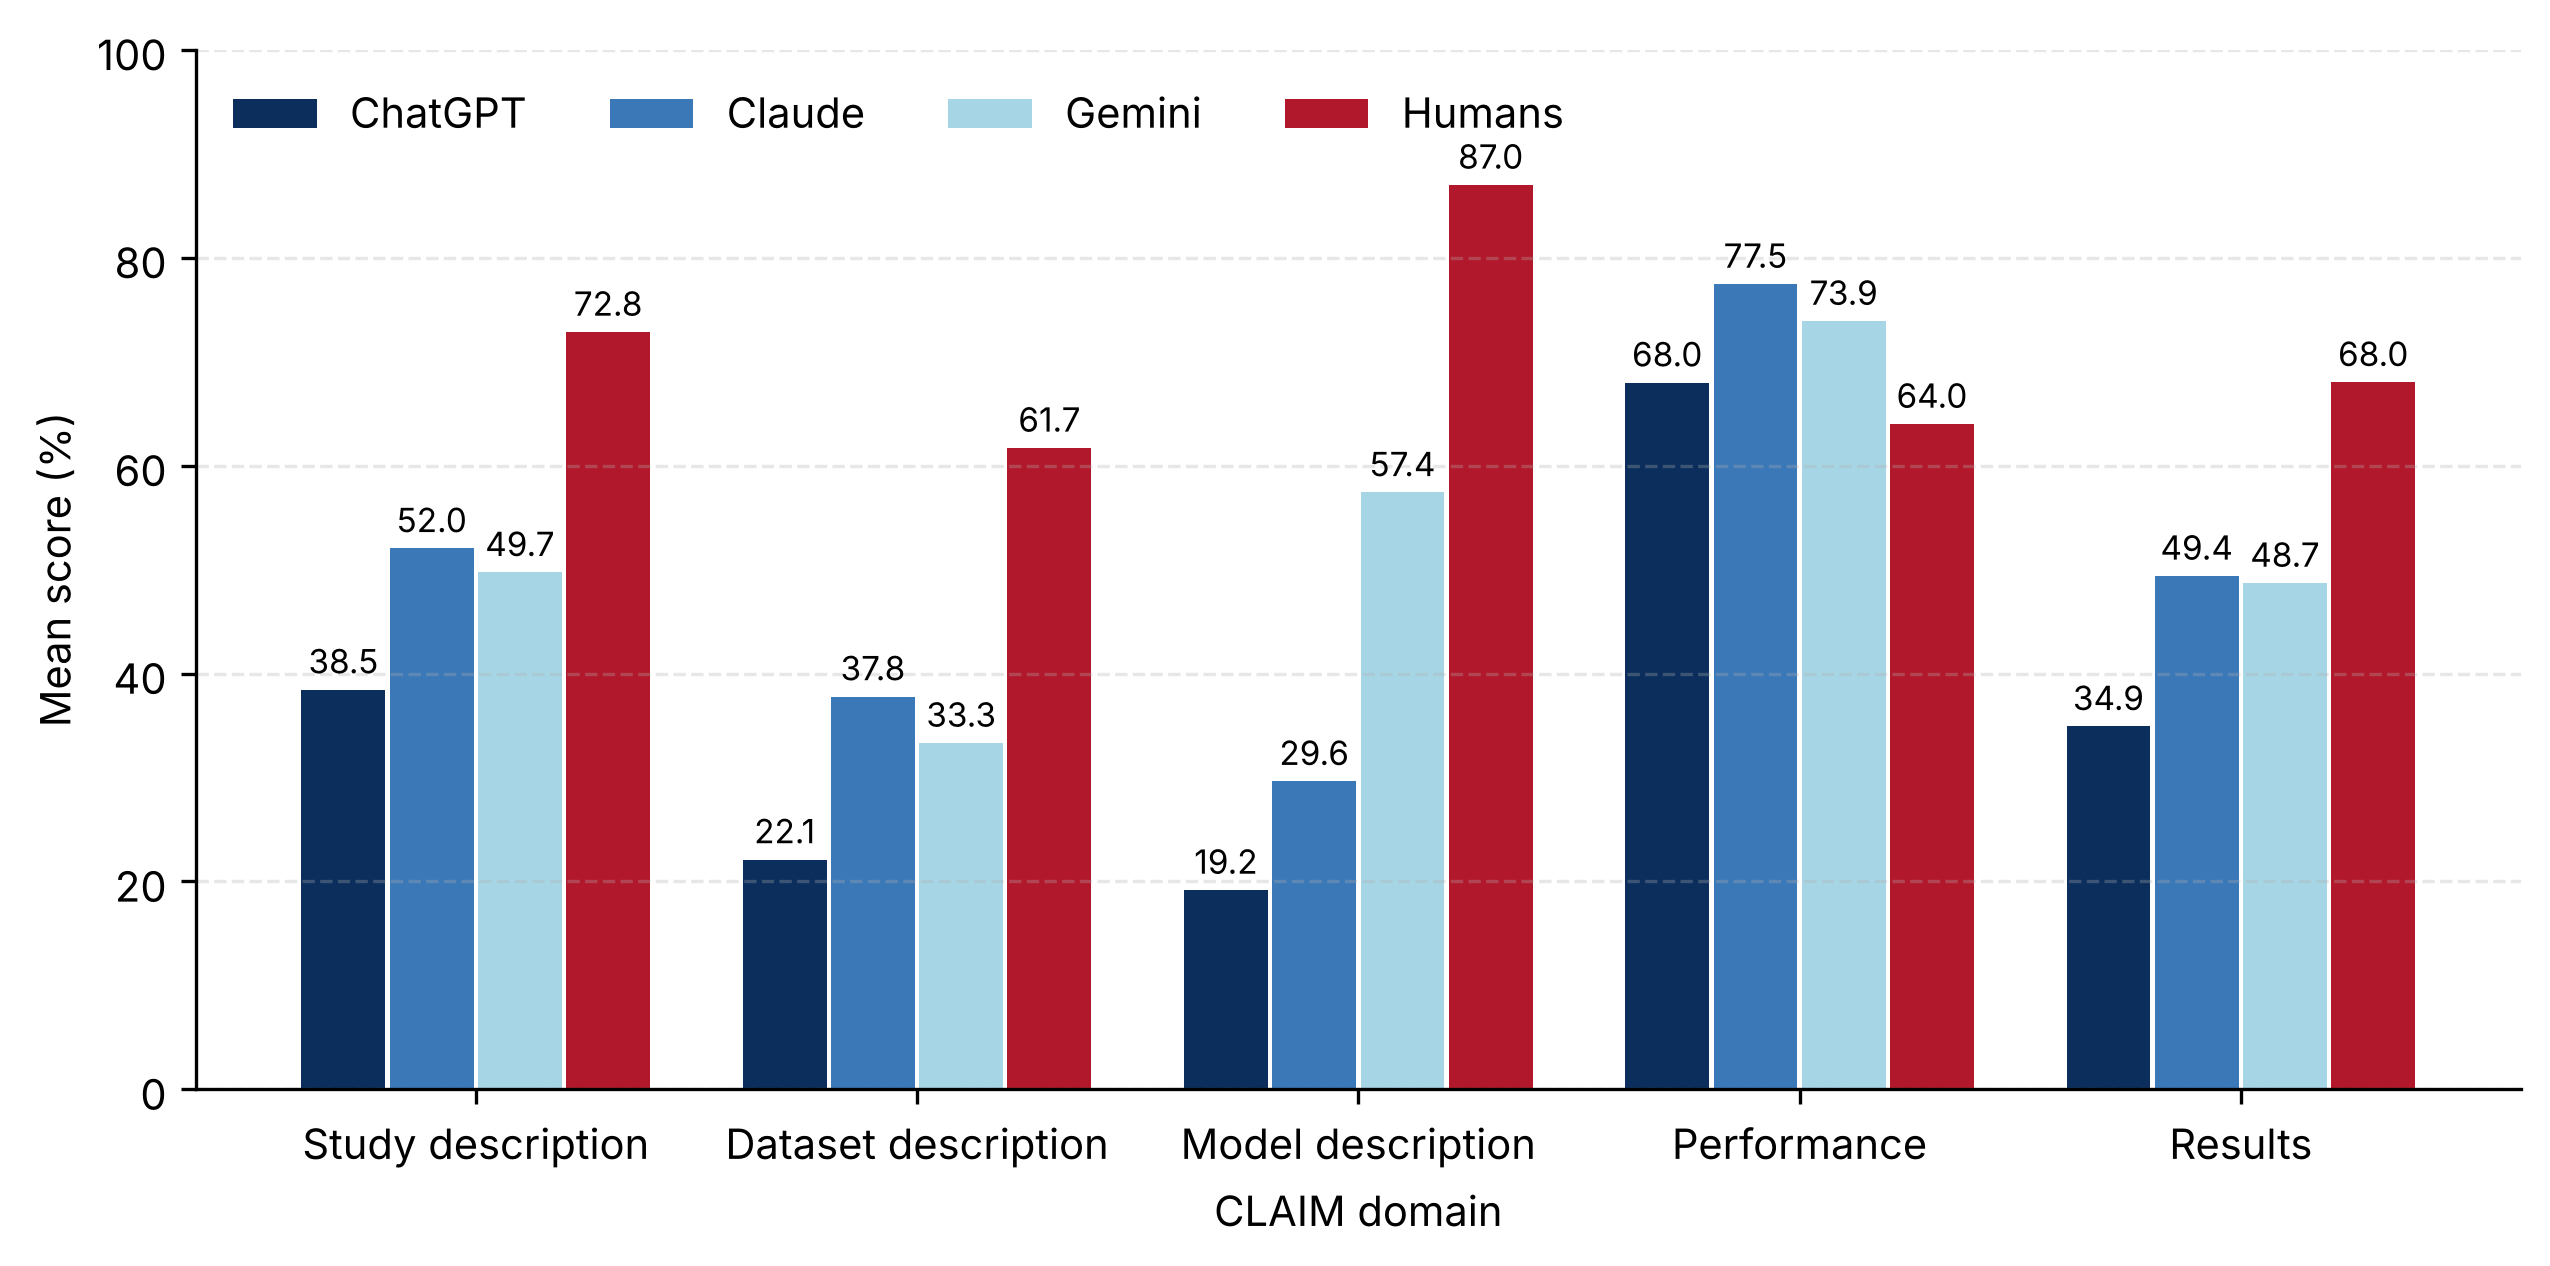
\includegraphics[height=3cm]{images/5ScoresDomain2.png}
        \caption{}
        \label{fig:scoreDomain}
    \end{subfigure}
    \caption{Comparison of CLAIM scores assigned by human and LLM evaluators. (a) Distribution of overall scores. (b) Mean scores across assessment domains.}
    \label{fig:scoreComparison}
\end{figure}
\vspace{-0.5cm}
\noindent
Additionally, evaluation scores were also examined across study metadata variables, ranging from ~10\% to 90\% with unequal sample sizes per category (Appendix \ref{app:scatterplot}). Across all variables, human scores remained consistently clustered at higher values, whereas LLM scores showed wider dispersion and variable overlap. 

\subsection{Agreement and strictness of LLMs compared to human evaluations}
As it can be seen in Table \ref{tab:mae_wilcoxon}, in three of the four CLAIM domains, all LLMs were significantly stricter than human reviewers (ME: $-18.6$ to $-67.8$ pp), with the largest discrepancies in Model description (MAE: 68.5, 61.9, and 42.5 for ChatGPT, Claude, and Gemini, respectively). Claude showed the lowest MAE in Results (21.7), whereas ChatGPT showed the highest (33.13). In Performance, Claude and Gemini were significantly more lenient (ME = 13.5 and 9.9 pp), while ChatGPT showed no significance (ME = 4.0 pp). Overall, 12 of 15 model domain comparisons showed negative bias, and 14 of 15 biases were statistically significant after multiple-comparison correction.
\vspace{-0.5cm}
\begin{table}[H]
\centering
\caption{MAE, ME and Wilcoxon test results comparing LLM and human scores.}
\label{tab:mae_wilcoxon}
\footnotesize
\setlength{\tabcolsep}{6pt}
\renewcommand{\arraystretch}{1.3}
\resizebox{\textwidth}{!}{
\begin{tabular}{llrrrrl}
\hline
\textbf{Target} & \textbf{Model} & \textbf{MAE} & \textbf{ME} &
\textbf{Wilcoxon p} & \textbf{Adjusted p} & \textbf{Direction} \\
\hline
Study description & ChatGPT & 34.600 & -34.400 & $3.58 \times 10^{-11}$ & $4.66 \times 10^{-10}$ & Stricter \\
Study description & Claude  & 25.383 & -20.817 & $1.39 \times 10^{-7}$  & $9.75 \times 10^{-7}$ & Stricter \\
Study description & Gemini  & 29.083 & -23.117 & $1.43 \times 10^{-7}$  & $9.75 \times 10^{-7}$ & Stricter \\
\hline
Dataset description & ChatGPT & 39.700 & -39.600 & $1.79 \times 10^{-11}$ & $2.68 \times 10^{-10}$ & Stricter \\
Dataset description & Claude  & 26.983 & -23.917 & $4.89 \times 10^{-9}$  & $4.89 \times 10^{-8}$ & Stricter \\
Dataset description & Gemini  & 35.150 & -28.383 & $5.71 \times 10^{-8}$  & $4.57 \times 10^{-7}$ & Stricter \\
\hline
Model description & ChatGPT & 68.500 & -67.833 & $6.44 \times 10^{-11}$ & $7.73 \times 10^{-10}$ & Stricter \\
Model description & Claude  & 61.900 & -57.367 & $5.26 \times 10^{-10}$ & $5.79 \times 10^{-9}$ & Stricter \\
Model description & Gemini  & 42.483 & -29.583 & $1.38 \times 10^{-5}$  & $5.53 \times 10^{-5}$ & Stricter \\
\hline
Performance & ChatGPT & 20.517 & 3.983 & $2.18 \times 10^{-1}$ & $2.18 \times 10^{-1}$ & More lenient \\
Performance & Claude  & 25.300 & 13.467 & $8.11 \times 10^{-4}$ & $2.43 \times 10^{-3}$ & More lenient \\
Performance & Gemini  & 22.200 & 9.900 & $4.84 \times 10^{-3}$ & $9.69 \times 10^{-3}$ & More lenient \\
\hline
Results & ChatGPT & 33.133 & -33.100 & $2.50 \times 10^{-11}$ & $3.50 \times 10^{-10}$ & Stricter \\
Results & Claude  & 21.700 & -18.633 & $2.64 \times 10^{-8}$  & $2.37 \times 10^{-7}$ & Stricter \\
Results & Gemini  & 24.850 & -19.317 & $2.18 \times 10^{-7}$  & $1.09 \times 10^{-6}$ & Stricter \\
\hline
\end{tabular}
}
\end{table}
\vspace{-0.5cm}

\subsection{Model differences}
Friedman test results from Table \ref{tab:freidman} revealed significant differences between LLMs in three of the four domains and in the overall score (all adjusted p < 0.001), with no significant difference in Performance (adjusted p = 0.052). Pairwise comparisons showed that Claude was significantly closer to human assessments than ChatGPT in Study description, Dataset description, and Results; and closer than Gemini in Dataset description. Gemini was closer to humans than both ChatGPT and Claude in Model description and closer than ChatGPT in Results. 
\vspace{-0.5cm}
\begin{table}[H]
\centering
\caption{Friedman test results comparing LLM scores across CLAIM domains.}
\label{tab:freidman}
\begin{tabular}{lccc}
\hline
\textbf{Domain} & \textbf{Friedman $\chi^2$} & \textbf{Adjusted p} & \textbf{Significant pairwise comparisons} \\
\hline
Study description   & 16.58 & $<0.001$ & ChatGPT vs \textbf{Claude} \\
Dataset description & 25.93 & $<0.001$ & ChatGPT vs \textbf{Claude}, \textbf{Claude} vs Gemini\\
Model description   & 20.79 & $<0.001$ & ChatGPT vs \textbf{Gemini}, Claude vs \textbf{Gemini} \\
Performance         & 5.93  & 0.052    & None  \\
Results             & 32.67 & $<0.001$ & ChatGPT vs \textbf{Claude}, ChatGPT vs \textbf{Gemini}\\
\hline
\end{tabular}
\begin{minipage}{\textwidth}
\vspace{2mm}
\footnotesize{\textit{Note.} The model in bold is the one more similar to human assessments in each pairwise comparison.}
\end{minipage}
\end{table}
\subsection{Rank correlation}
Spearman correlations of Figure \ref{fig:Spearman} showed no significant association between any LLM and the human evaluations in any CLAIM domain ($(\rho)$ between -0.29 and 0.02), indicating that the LLMs did not rank papers in the same order as human reviewers. The weakest correlations were observed for Dataset description (Gemini, $(\rho)$ = -0.29) and Results (Gemini, $(\rho)$ = -0.27). 

In contrast, agreement among LLMs was higher, with 6 of the 15 pairwise correlations being significant after multiple-testing adjustment. It was strongest between ChatGPT and Claude in Study description ($(\rho)$ = 0.65), Dataset description ($(\rho)$ = 0.62) and Results ($(\rho)$ = 0.54), while Model description showed the lowest agreement ($(\rho)$ = 0.13-0.33, none significant). 
\vspace{-0.5cm}
\begin{figure}[H]
    \centering
    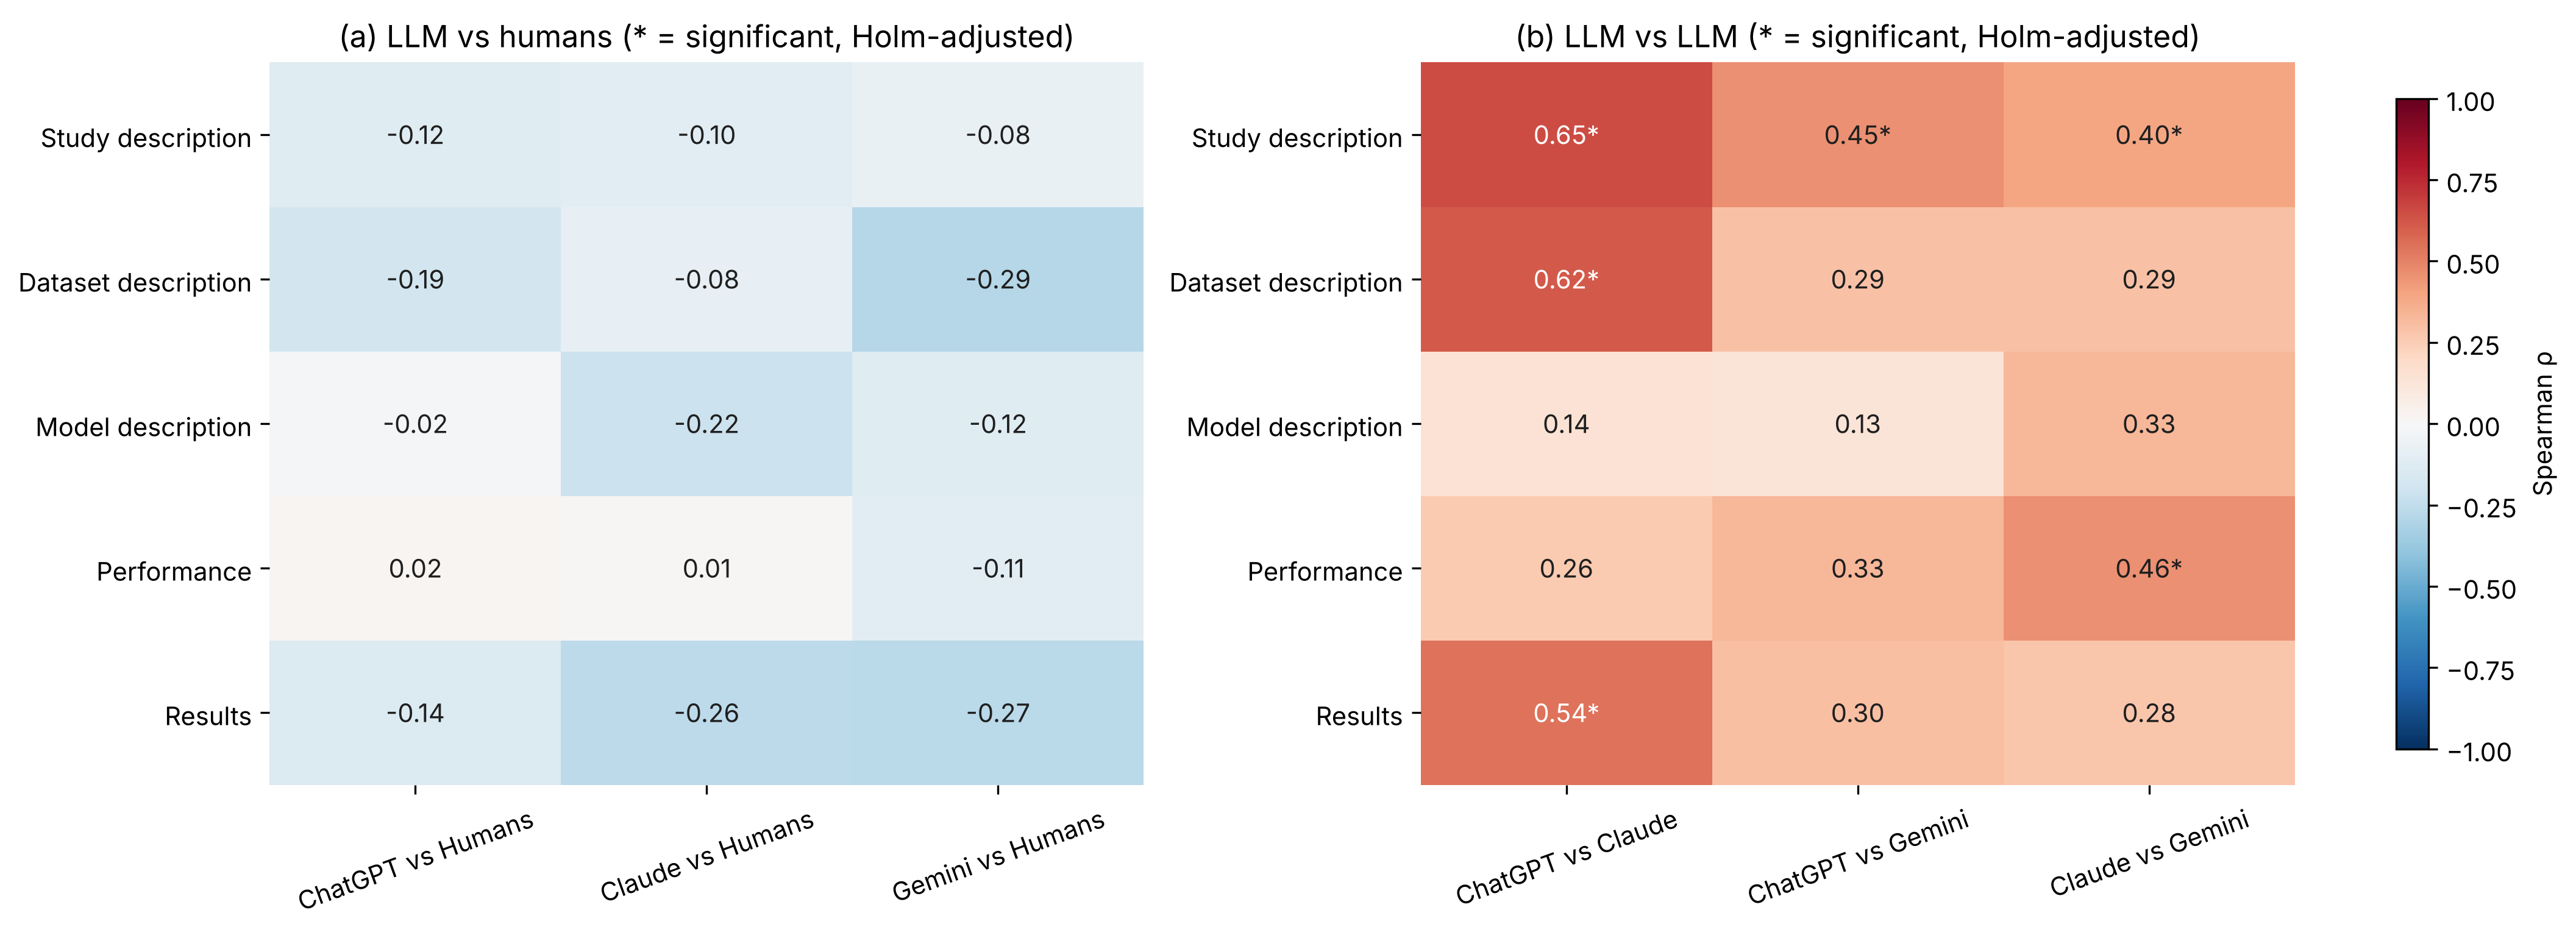
\includegraphics[width=0.9\linewidth]{images/2Spearmanrho.png}
    \caption{Spearman correlation coefficients across CLAIM domains for (a) LLM and human assessments and (b) pairs of LLMs.}
    \label{fig:Spearman}
\end{figure}
\vspace{-0.5cm}


%\begin{figure}[H]
%    \centering
%    \includegraphics[width=1\linewidth]{images/6Metadataresults2.png}
%    \caption{Relationship between overall CLAIM evaluation scores and selected study metadata (performance evaluation, public code availability and link type), stratified by evaluator. Each point represents an individual assessment, with colours distinguishing evaluators.}
%    \label{fig:Metadata}
%\end{figure}

